\chapter{Технологический раздел}

В данном разделе будут выбраны СУБД, средства реализации приложения, описано создание базы данных, триггера, ролей с последующим выделением прав, наполнение базы, а также спроектирован пользовательский интерфейс.

\section{Выбор СУБД}

В настоящее время существует множество систем управления базами данных, работающих на основе реляционной модели. Среди самых распространенных \cite{most_popular} выделяют MySQL \cite{mysql}, PostgreSQL \cite{postgresql} и замыкает тройку лидеров SQLite \cite{sqlite}. Рассмотрим особенности каждой из них.
\begin{enumerate}
	\item MySQL. Среди достоинств данной СУБД можно выделить простой синтаксис, высокую безопасность и масштабируемость, поддержку большей части функционала SQL. Однако, несмотря на перечисленные положительные аспекты, MySQL сильно подвергается DDos-атакам и не сопровождается бесплатной технической поддержкой.
	\item PostgreSQL. В рамках использования этой СУБД имеется возможность помимо встроенного SQL использовать различные дополнения, отличается поддержкой форматов csv и json, но оперирует большим объемом ресурсов.
	\item SQLite. Очевидными достоинствами является компактность базы данных, которая состоит из одного файла, и легкая переносимость. Но данная СУБД совершенно не подходит для больших БД, а также не поддерживает управление пользователями.
\end{enumerate}

При реализации проекта будет использован PostgreSQL, поскольку эта СУБД обладает достаточным набором инструментов для поставленной задачи.

%При реализации будет использован PostgreSQL, так как он уже использовался в ранее изученном курсе.

\section{Средства реализации}

В качестве используемого языка программирования выбрана Java \cite{java}, так как:
\begin{itemize}
	\item данный язык является объектно-ориентированным, позволяя использовать наследование, интерфейсы, абстракции и т.~д.;
	\item имеет JDBC \cite{jdbc} -- API для выполнения SQL-запросов к базам данных.
\end{itemize}

В качестве среды разработки используется IntelliJ IDEA \cite{intellij_idea}, поскольку данная программа:
\begin{itemize}
	\item имеет удобный интерфейс взаимодействия и подключения используемых зависимостей;
	\item предоставляет возможности тестирования и запуска написанного приложения с определенными файлами конфигурации.
\end{itemize}

\section*{Создание базы данных}

В соответствии с выбранной СУБД и спроектированной базой данных было осуществлено создание БД и ее сущностей. Реализация представлена в приложении А, листинг \ref{create}.

\section{Создание триггера}

В предыдущем разделе был спроектирован триггер AFTER на создание новой заявки в системе. Код его создания представлен в листинге \ref{trigger_code}

\captionsetup{singlelinecheck = false, justification=raggedright}
\begin{lstlisting}[language=sql, caption=Реализация триггера AFTER на добавление заявки, label=trigger_code]
create trigger newRequest
after insert 
on sosedushka_db.request 
for each row 
execute function checkBanWords()
\end{lstlisting}
\captionsetup{singlelinecheck = false, justification=centering}

Для этого триггера была написана соответствующая функция с помощью PL/pgSQL \cite{plpgsql} -- процедурного расширения языка SQL, используемого в СУБД PostgreSQL. Код функции представлен в листинге \ref{trigger_func}.

\captionsetup{singlelinecheck = false, justification=raggedright}
\begin{lstlisting}[language=sql, caption=Реализация функции checkBanWords(), label=trigger_func]
create or replace function checkBanWords()
returns trigger as 
$$
declare 
	banWords text ARRAY;
begin 
	banWords := ARRAY(select '%' || word || '%' from sosedushka_db.ban);
	if new.title like any (banWords) or new.explanation like any (banWords)
	then
		raise notice 'Bad words existing!';
		update sosedushka_db.request set status='BANNED' where id=new.id;
		return null;
	else
		return new;
	end if;
end
$$
language plpgsql
\end{lstlisting}
\captionsetup{singlelinecheck = false, justification=centering}

\section{Создание ролей и выделение им прав}

В конструкторском разделе была разработана ролевая модель, в которой выделены следующие роли:
\begin{itemize}
	\item customer -- оформитель заявки;
	\item executor -- исполнитель заявки;
	\item administrator -- администратор.
\end{itemize}

Соответствующий этой ролевой модели сценарий создания ролей и выделения им прав представлен на листинге \ref{roles}.\newpage

\captionsetup{singlelinecheck = false, justification=raggedright}
\begin{lstlisting}[language=sql, caption=Создание ролей и выделение им прав, label=roles]
create role customer with login password '1111';
grant insert, update on table sosedushka_db.user to customer;
grant insert, update on table sosedushka_db.connection to customer;
grant all privileges on table sosedushka_db.request to customer;
grant insert on table sosedushka_db.skill to customer;
grant insert on table sosedushka_db.equipment to customer;

create role executor with login password '2222';
grant insert, update on table sosedushka_db.user to executor;
grant insert, update on table sosedushka_db.connection to executor;
grant select, update on table sosedushka_db.request to executor;
grant insert on table sosedushka_db.skill to executor;
grant insert on table sosedushka_db.executorskill to executor;

create role administrator with login password '4813';
grant all privileges on table sosedushka_db.user to administrator;
grant all privileges on table sosedushka_db.connection to administrator;
grant all privileges on table sosedushka_db.executorskill to
administrator;
grant all privileges on table sosedushka_db.ban to administrator;
\end{lstlisting}
\captionsetup{singlelinecheck = false, justification=centering}

\section{Наполнение базы данных}

Каждая из описанных сущностей (за исключением таблицы Ban) была заполнена 1000 значений. Рассмотрим каким образом осуществлялась генерация данных.
\begin{enumerate}
	\item Таблица User -- все значения получены случайным образом в соответствии с описанными типами данных полей.
	\item Таблица Connection -- для каждого пользователя из таблицы User текущая роль выбиралась случайным образом из сгенерированных доступных ему ролей.
	\item Таблицы Equipment и Skill -- значения были получены путем поиска в интернете различных подходящих для таблиц значений.
	\item Таблица ExecutorSkill -- для каждого случайно выбранного пользователя из таблицы User со значением поля executorRole = True случайным образом выбирался навык из таблицы Skill и статус навыка из перечня доступных.
	\item Таблица Request -- заголовок, пояснение и статус выбирались случайно из списка доступных, срок актуальности заполнен одинаковым значением, оформитель и исполнитель выбраны случайным образом из таблицы User с проверкой соответствующих ролей, навык и оборудование выбирались таким образом, чтобы области применения оборудования не противоречили с областью применения навыка.
\end{enumerate}

Значения таблицы Ban были получены путем выделения основ нецензурных слов. Итоговый объем составил 50 записей. 

Выгрузка значений из электронных таблиц в базу данных представлен в приложении А, листинг \ref{fill}.

\section{Интерфейс приложения}

Для работы с базой данных был разработан интерфейс взаимодействия в виде telegram-бота. 

В поле поиска чатов необходимо ввести @Sosed\_Ushka\_Bot, перейдя в этот диалог можно увидеть приветственное сообщение и ввести команду $/start$. После этого будет предложено пройти персонализацию командой $/personalize$ под одной из имеющихся ролей. На рисунке \ref{personalize} представлена иллюстрация вышеописанных действий и персонализация под ролью оформителя.

% На рисунках \ref{personalize}-\ref{administrator} представлены примеры персонализации, взаимодействия с системой оформителя, исполнителя и администратора. 

\begin{figure}[H]
	\begin{center}
		%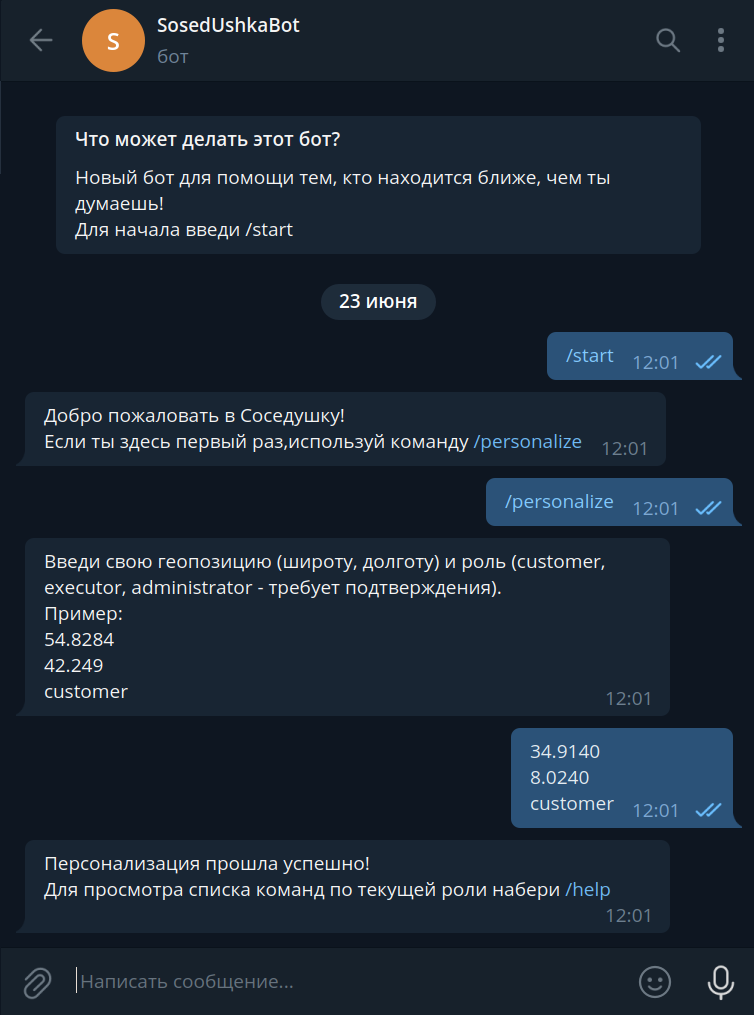
\includegraphics[scale=0.3]{assets/personalize.png}
		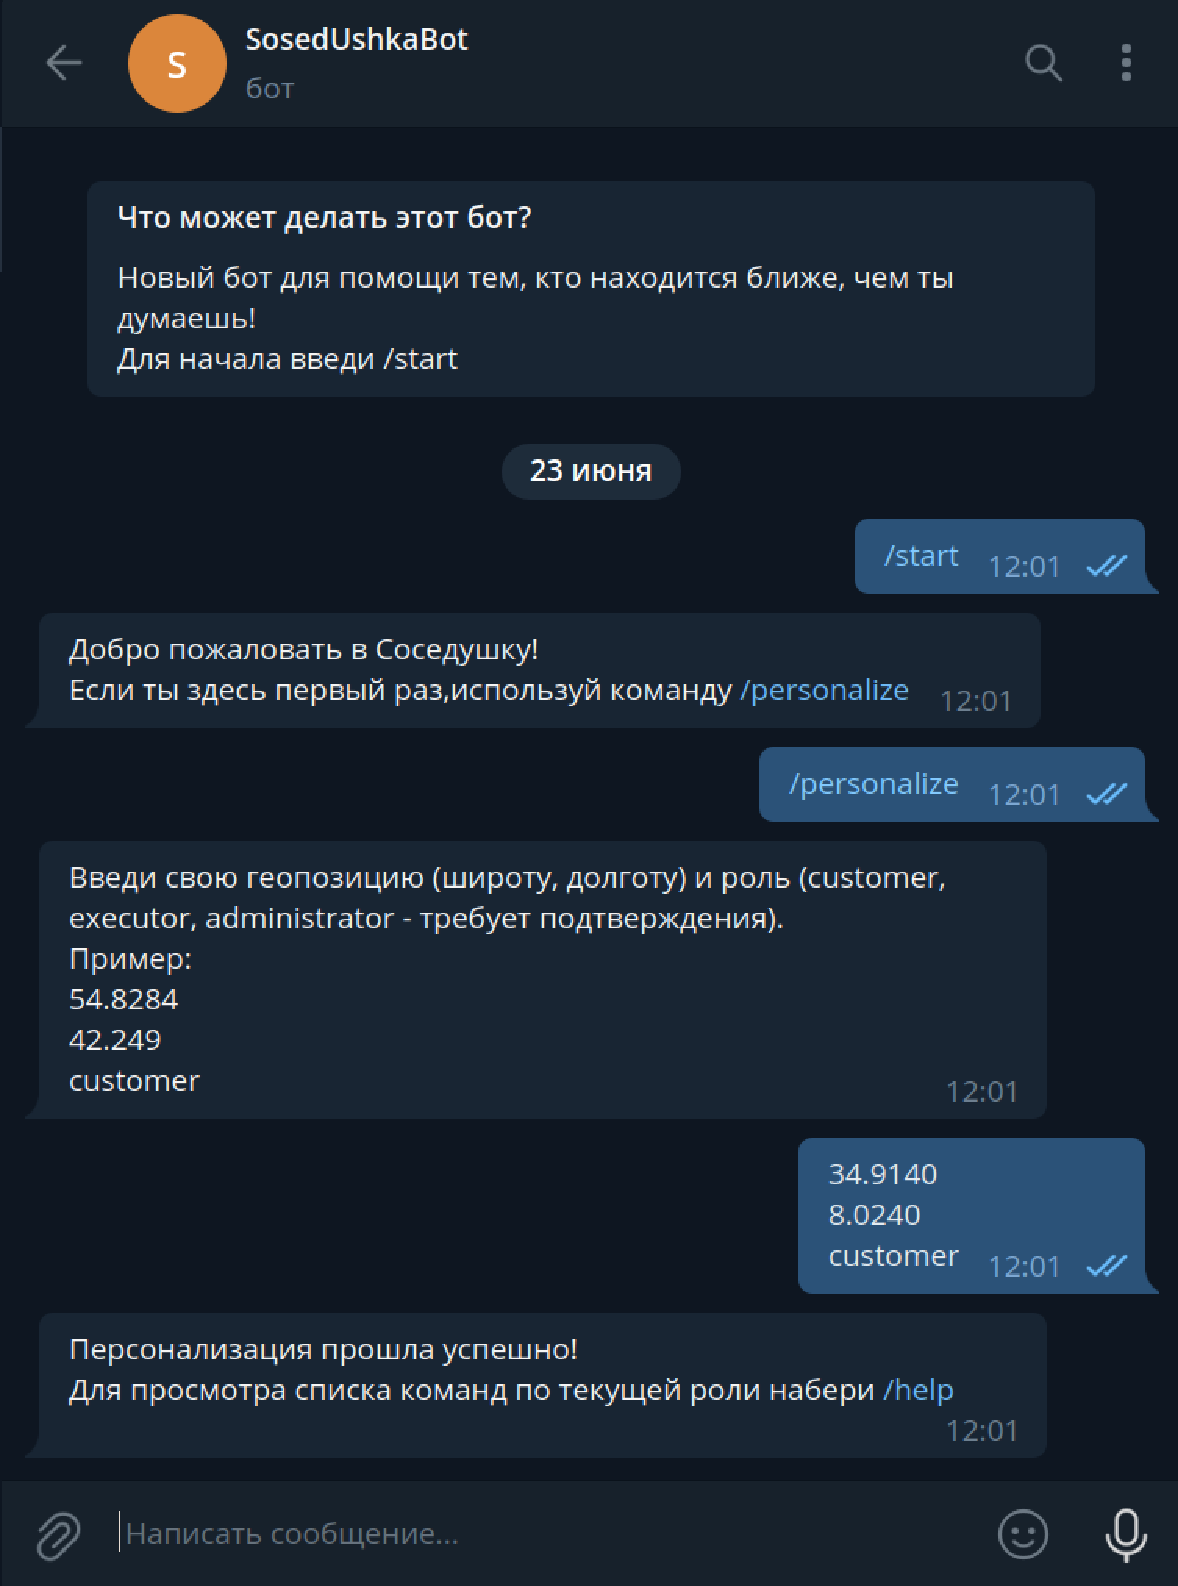
\includegraphics[page=1,scale=0.4]{assets/personalize.pdf}
	\end{center}
	\caption{Интерфейс персонализации}
	\label{personalize}
\end{figure}

Чтобы увидеть список доступных команд для текущей роли можно ввести команду $/help$ (рисунок \ref{help_customer}). Также можно сменить геопозицию пользователя командой $/change\_geo$ (рисунок \ref{change_geo}).

\begin{figure}[H]
	\begin{center}
		%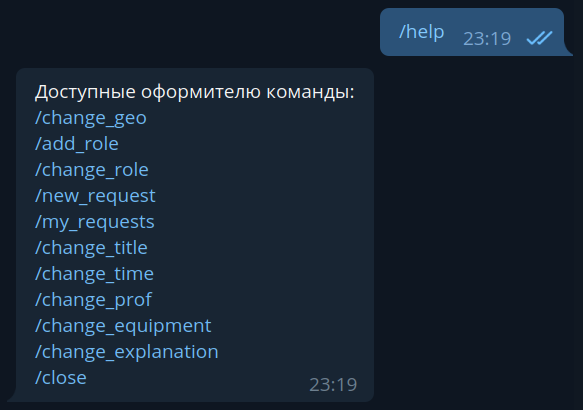
\includegraphics[scale=0.38]{assets/help_customer.png}
		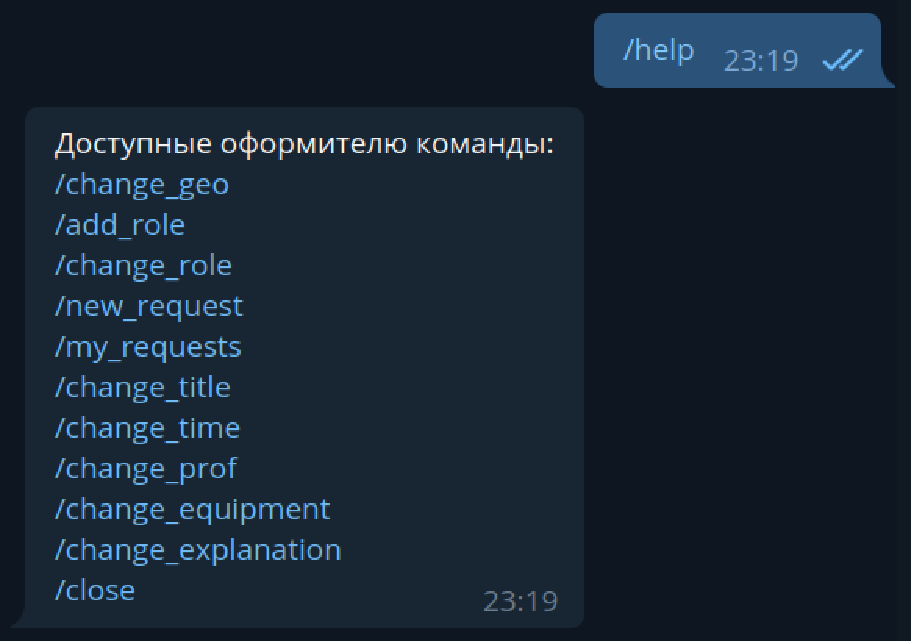
\includegraphics[page=1,scale=0.5]{assets/help_customer.pdf}
	\end{center}
	\caption{Интерфейс персонализации}
	\label{help_customer}
\end{figure}

\begin{figure}[H]
	\begin{center}
		%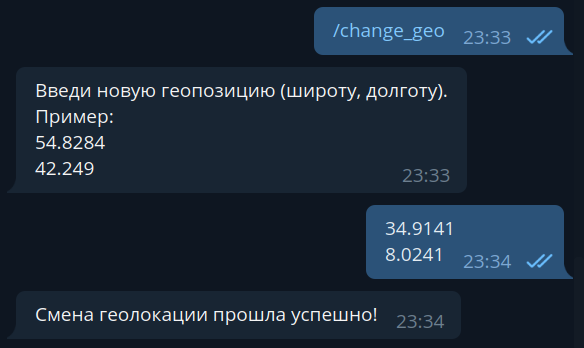
\includegraphics[scale=0.38]{assets/change_geo.png}
		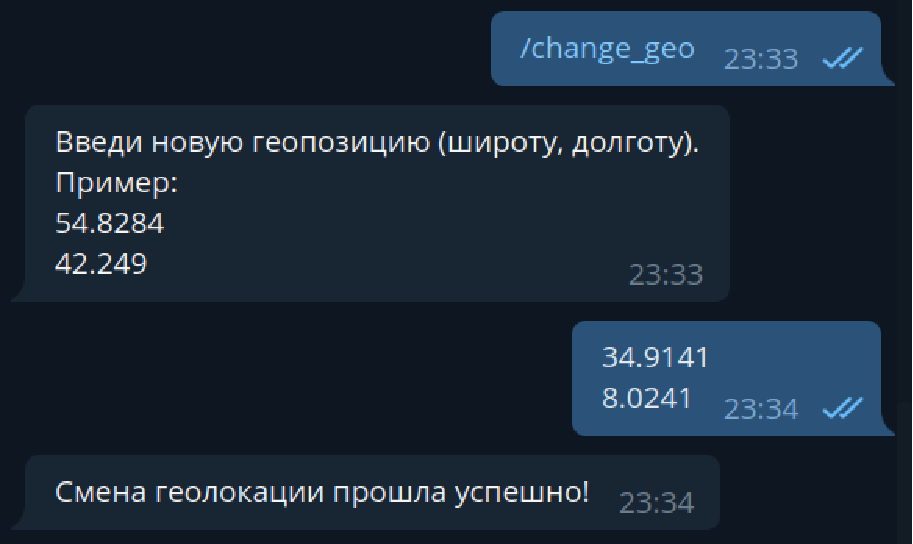
\includegraphics[page=1,scale=0.5]{assets/change_geo.pdf}
	\end{center}
	\caption{Интерфейс персонализации}
	\label{change_geo}
\end{figure}

Рассмотрим взаимодействие с заявками. Командой $/new\_request$ можно создать заявку, введя заголовок, время актуальности, пояснение, необходимый навык и оборудование. Ненужные поля можно оставить пустыми, кроме заголовка и актуальности. Командой $/my\_requests$ можно получить список открытых или исполняемых заявок. Иллюстрация описанных действий отображена на рисунке \ref{customer}.

\begin{figure}[H]
	\begin{center}
		%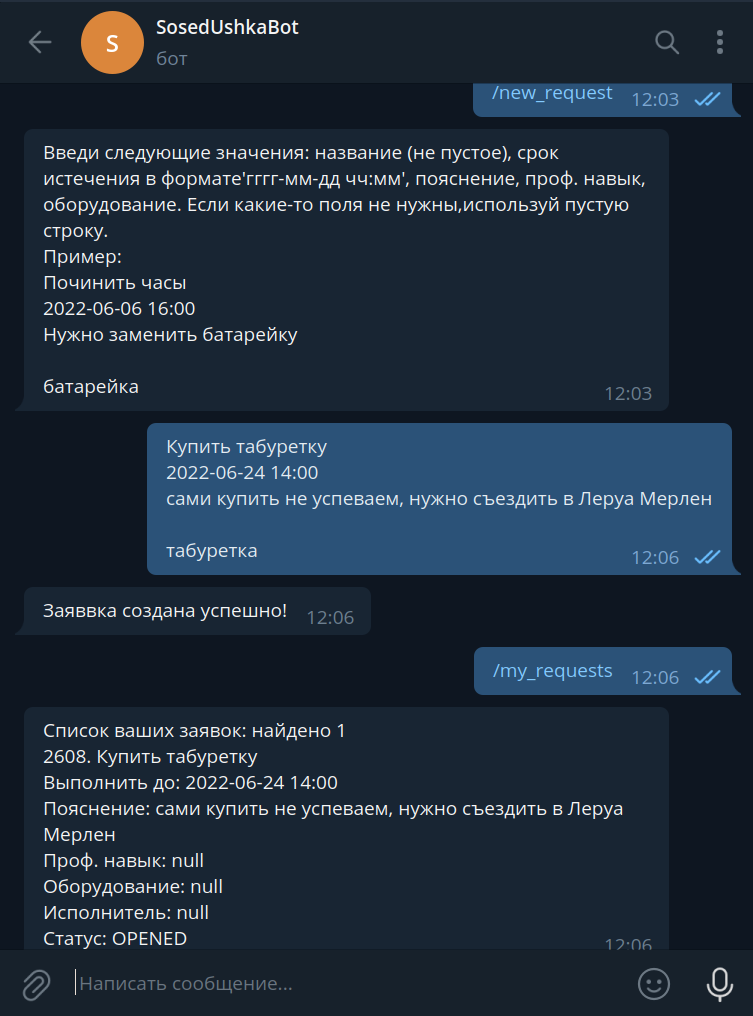
\includegraphics[scale=0.3]{assets/customer.png}
		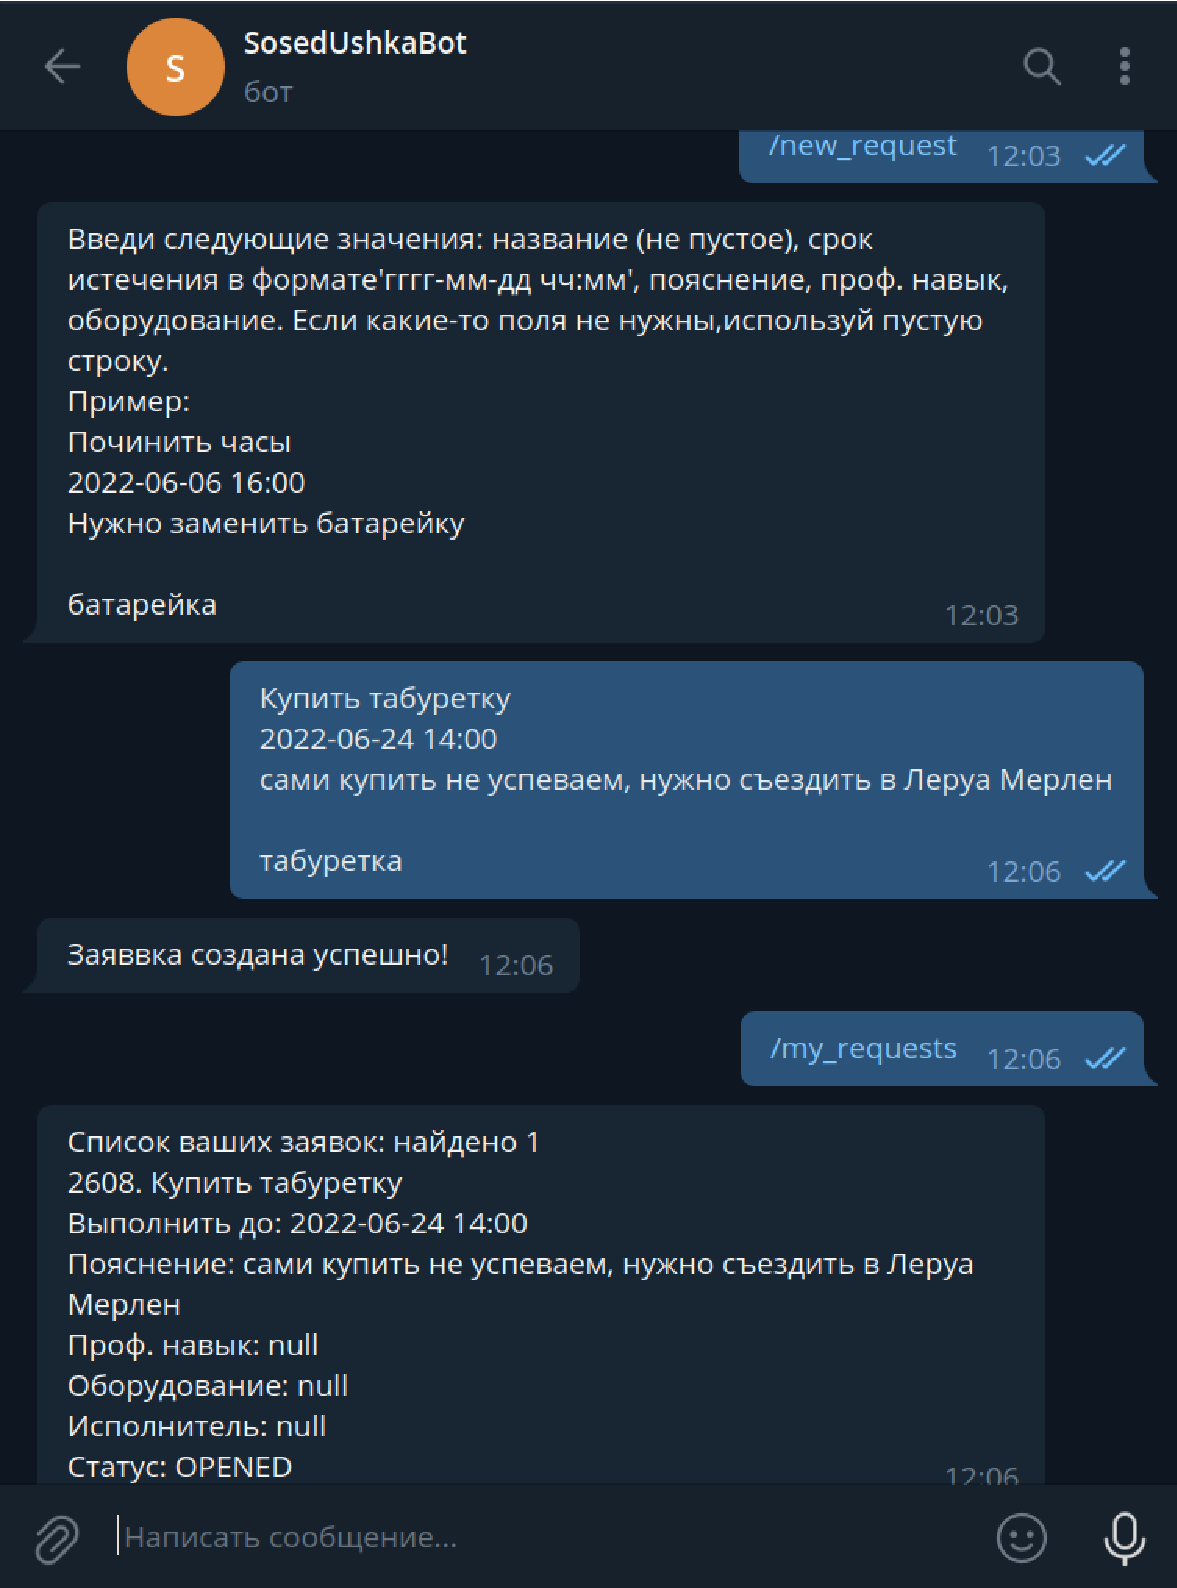
\includegraphics[page=1,scale=0.4]{assets/customer.pdf}
	\end{center}
	\caption{Интерфейс создания и просмотра списка заявок оформителя}
	\label{customer}
\end{figure}

Каждое из полей заявки можно изменить соответствующей командой. Например, пояснение изменяется использование $/change_explanation$. Также доступно закрытие заявки командой $/close$. Реализация на рисунке \ref{change_close}.

\begin{figure}[H]
	\begin{center}
		%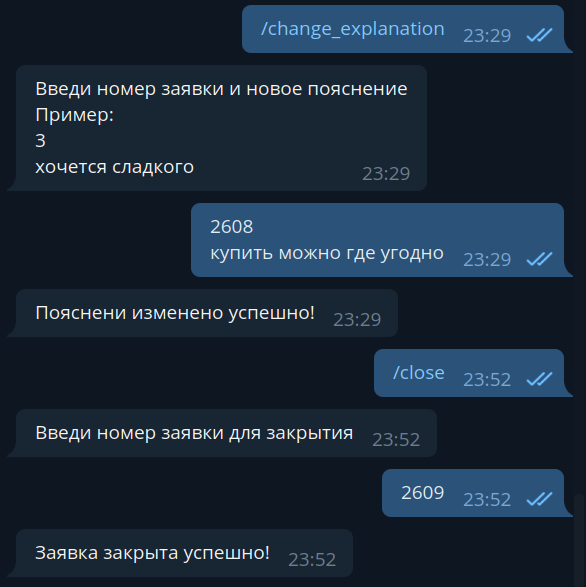
\includegraphics[scale=0.38]{assets/change_close.png}
		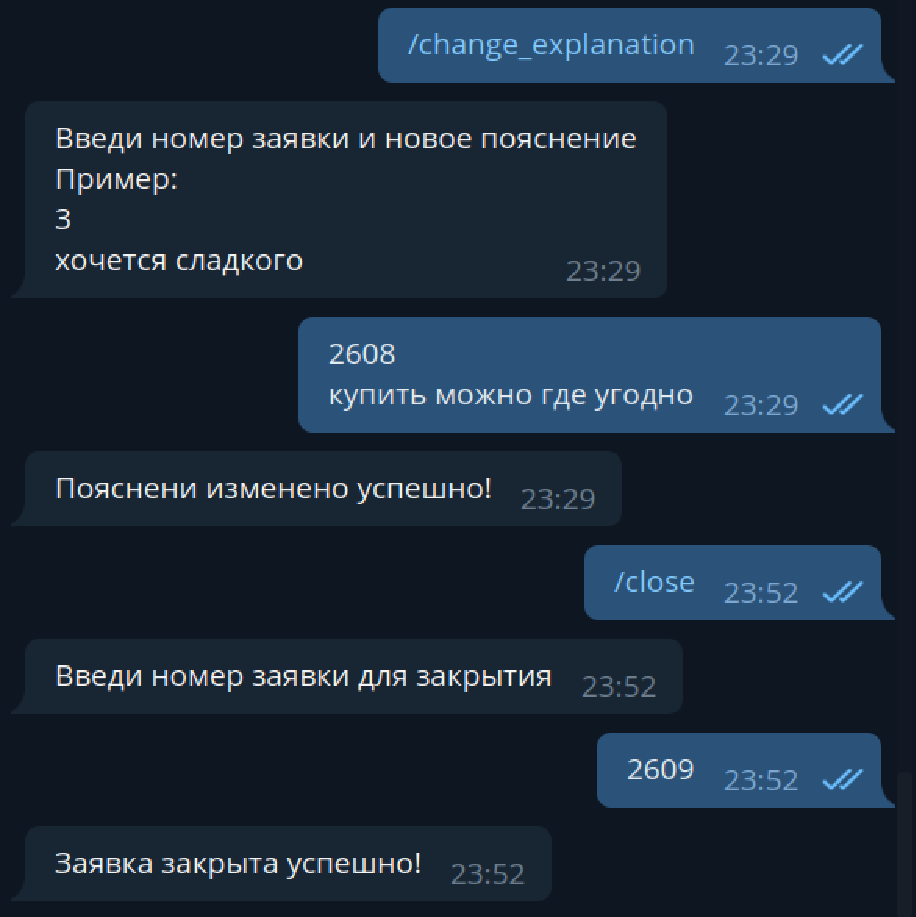
\includegraphics[page=1,scale=0.5]{assets/change_close.pdf}
	\end{center}
	\caption{Интерфейс изменения поля заявки и ее закрытия}
	\label{change_close}
\end{figure}

Также имеется возможность добавления роли и соответствующего перехода к ней. Рассмотрим на смену роли от оформителя к исполнителю. Командой $/add\_role$ добавляем пользователю роль executor, и переходим к ней командой $/change\_role$. После успешного перехода появится соответствующее сообщение (рисунок \ref{add_role}). 

\begin{figure}[H]
	\begin{center}
		%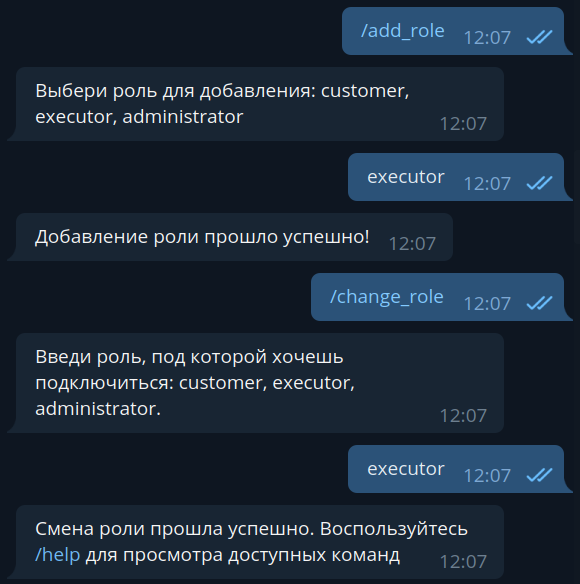
\includegraphics[scale=0.38]{assets/add_role.png}
		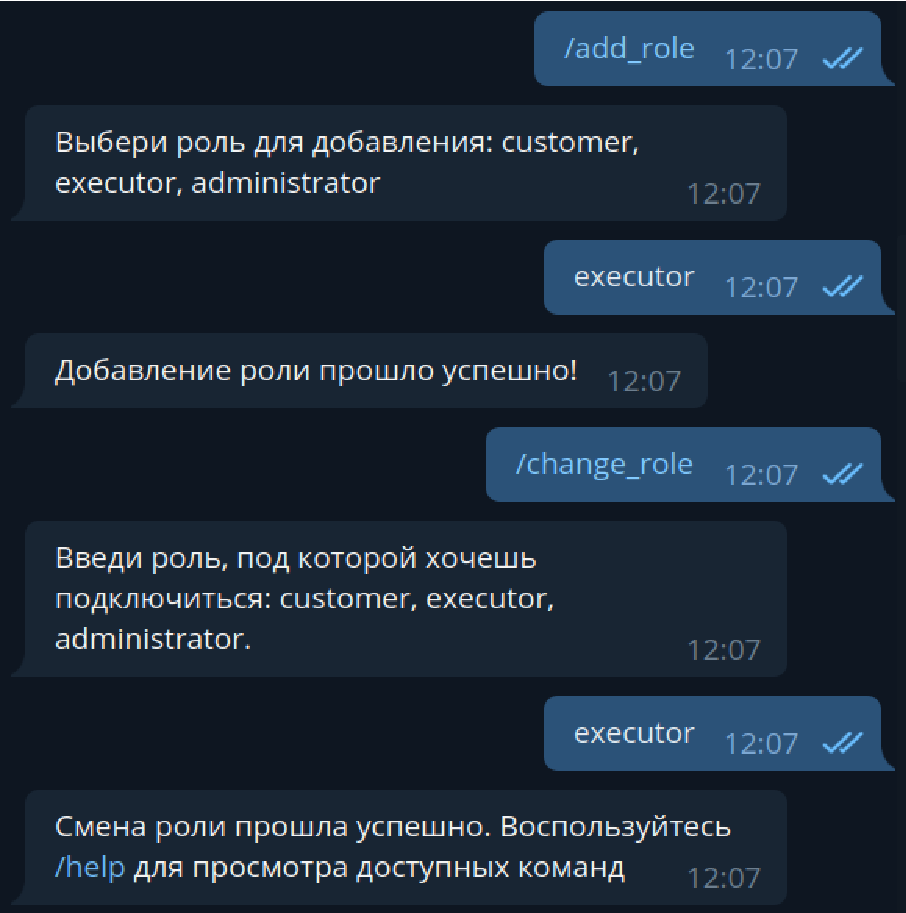
\includegraphics[page=1,scale=0.5]{assets/add_role.pdf}
	\end{center}
	\caption{Интерфейс добавления и смены роли}
	\label{add_role}
\end{figure}

Исполнитель может отправить свой навык на подтверждение администратора командой $/send\_to\_verify$ (рисунок \ref{send_to_verify}). Для этого необходимо ввести его название. Если навыка еще нет в базе, то он добавляется.

\begin{figure}[H]
	\begin{center}
		%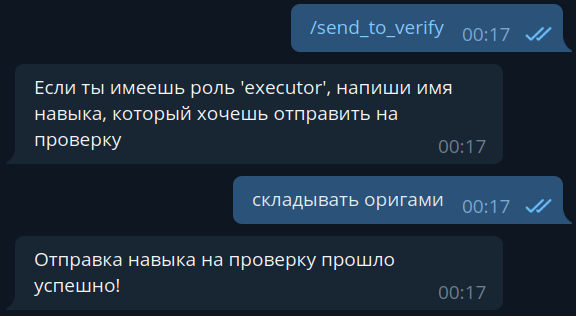
\includegraphics[scale=0.38]{assets/send_to_verify.png}
		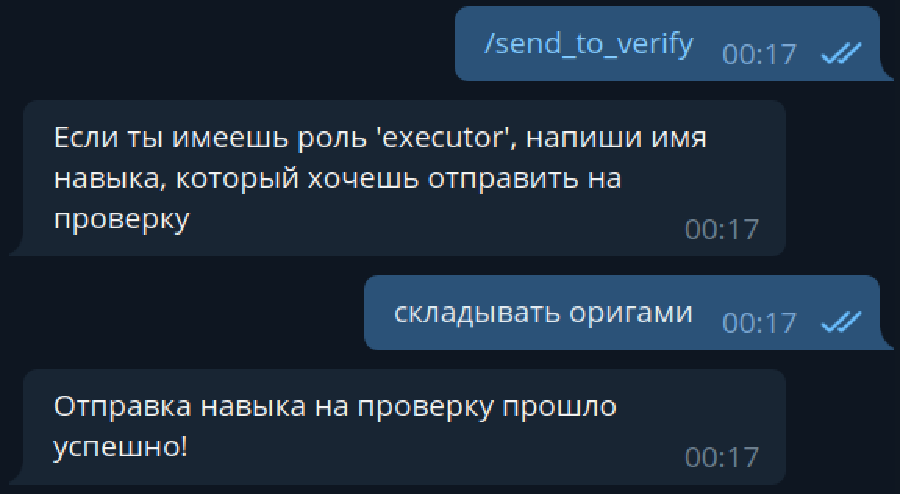
\includegraphics[page=1,scale=0.5]{assets/send_to_verify.pdf}
	\end{center}
	\caption{Интерфейс отправки навыка исполнителя на подтверждение}
	\label{send_to_verify}
\end{figure}

Имеется возможность просмотреть список подходящих по навыкам исполнителя заявок (в том числе без необходимого навыка), указывая необходимую дальность от своей геопозиции в километрах. Это делается командой $/get\_request\_on\_my\_skill$. Также можно взять одну из них на исполнение командой $/take$ (показано на рисунке \ref{take}).

\begin{figure}[H]
	\begin{center}
		%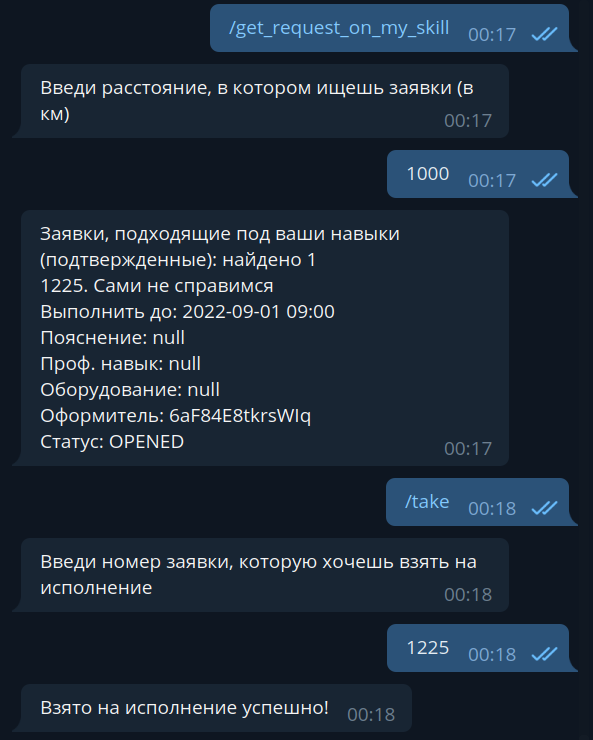
\includegraphics[scale=0.38]{assets/take.png}
		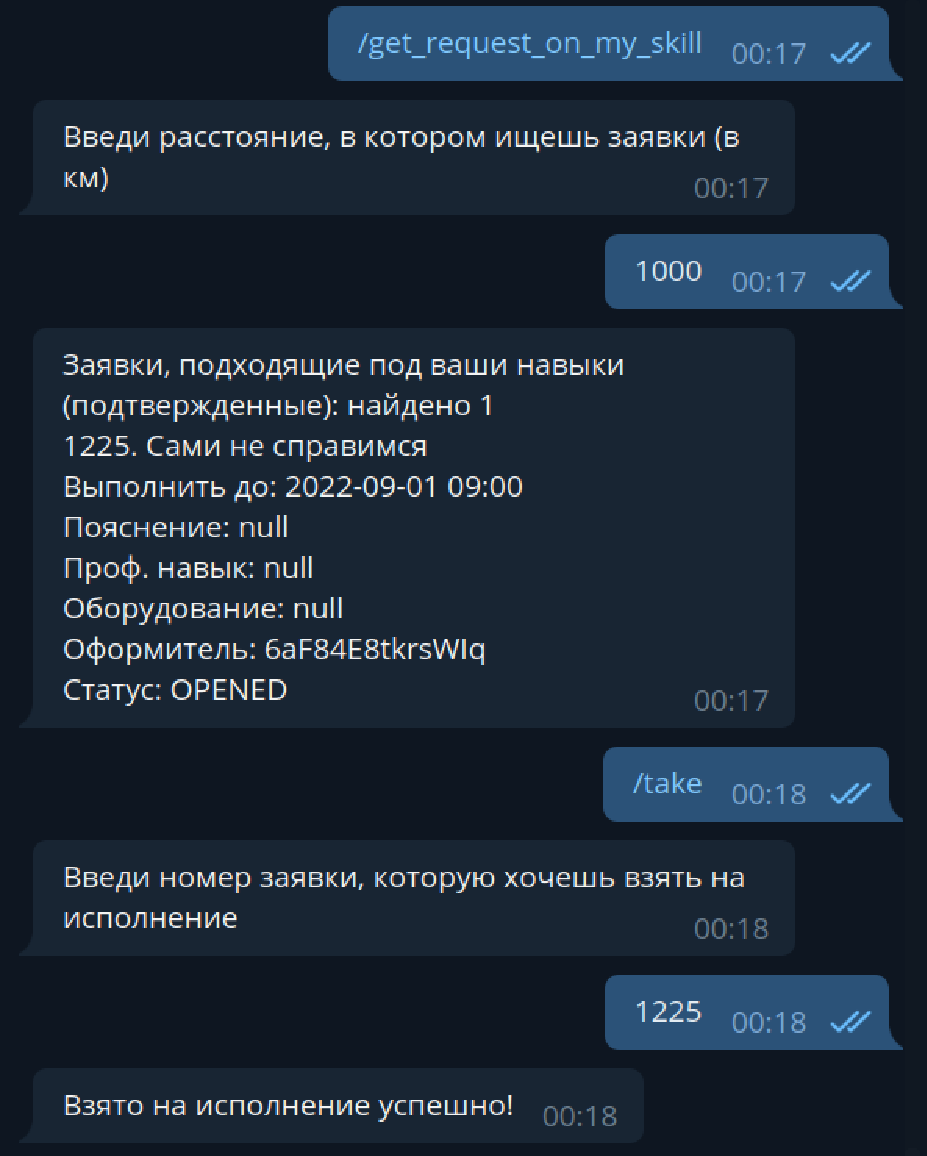
\includegraphics[page=1,scale=0.5]{assets/take.pdf}
	\end{center}
	\caption{Интерфейс просмотра заявок по навыку и взятия их на исполнение}
	\label{take}
\end{figure}

Когда заявка будет выполнена, исполнитель может перевести заявку в соответствующий статус командой $/done$ (рисунок \ref{done}).

\begin{figure}[H]
	\begin{center}
		%
\includegraphics[scale=0.38]{assets/done.png}
		
\includegraphics[page=1,scale=0.5]{assets/done.pdf}
	\end{center}
	\caption{Интерфейс перевода заявки в статус выполненной}
	\label{done}
\end{figure}

Перейдем к возможностям администратора. Добавление этой роли происходит не сразу, поэтому подключение под этой ролью будет доступно только после подтверждения (рисунок \ref{add_adm}).

\begin{figure}[H]
	\begin{center}
		%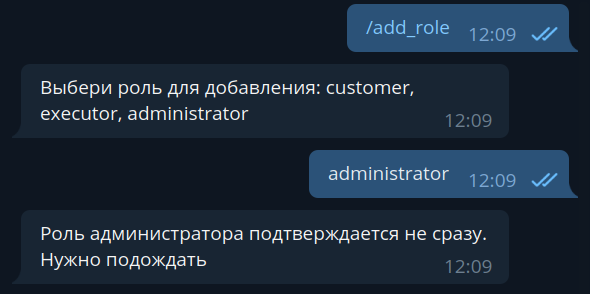
\includegraphics[scale=0.38]{assets/add_adm.png}
		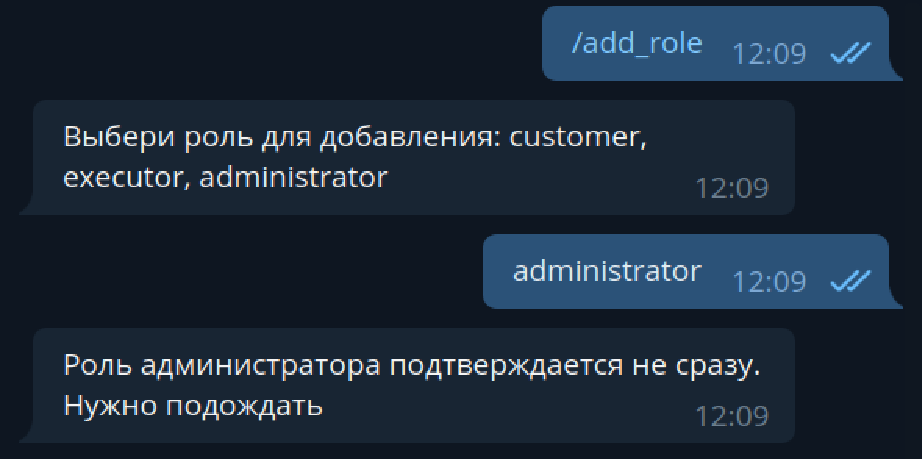
\includegraphics[page=1,scale=0.5]{assets/add_adm.pdf}
	\end{center}
	\caption{Интерфейс добавления роли администратора}
	\label{add_adm}
\end{figure}

Администратору доступно подтверждение навыков исполнителей командой $/skill\_verify$ с предварительным просмотром списка неподтвержденных, командой $/get\_skill\_to\_verify$. Пример работы на рисунке \ref{skill_verify}.

\begin{figure}[H]
	\begin{center}
		%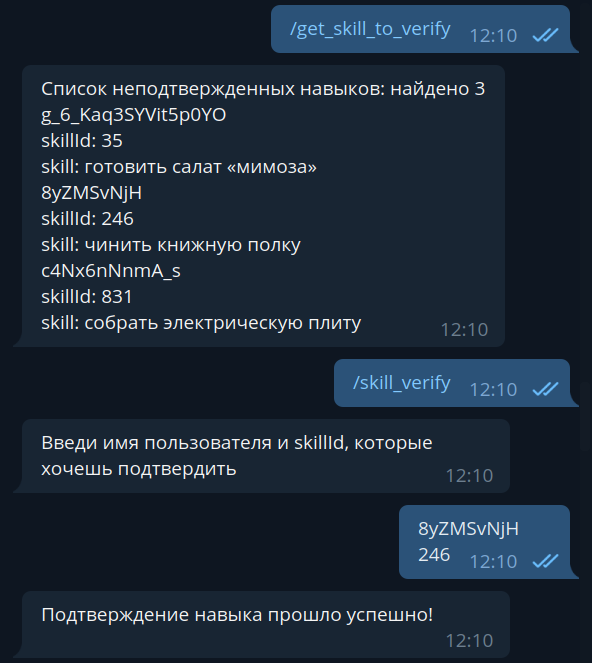
\includegraphics[scale=0.38]{assets/skill_verify.png}
		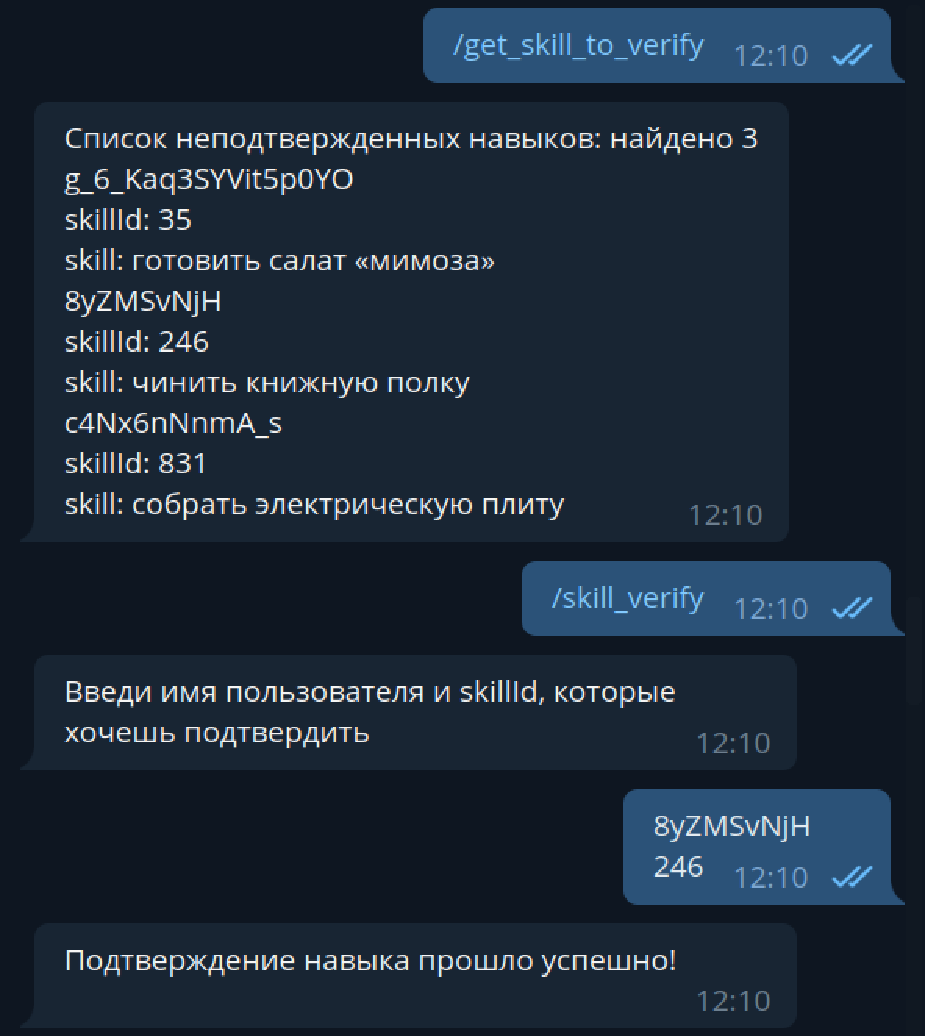
\includegraphics[page=1,scale=0.5]{assets/skill_verify.pdf}
	\end{center}
	\caption{Интерфейс подтверждения навыков исполнителей}
	\label{skill_verify}
\end{figure}

Аналогичный интерфейс доступен для просмотра неподтвержденных администраторов -- $/get\_admin\_to\_verify$ и $/admin\_verify$ (рисунок \ref{admin_verify}).

\begin{figure}[H]
	\begin{center}
		%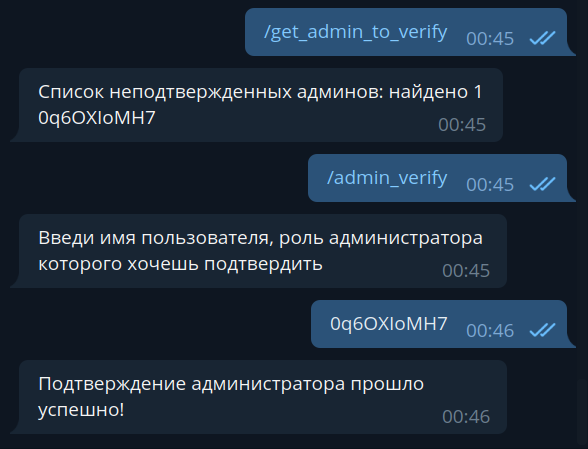
\includegraphics[scale=0.38]{assets/admin_verify.png}
		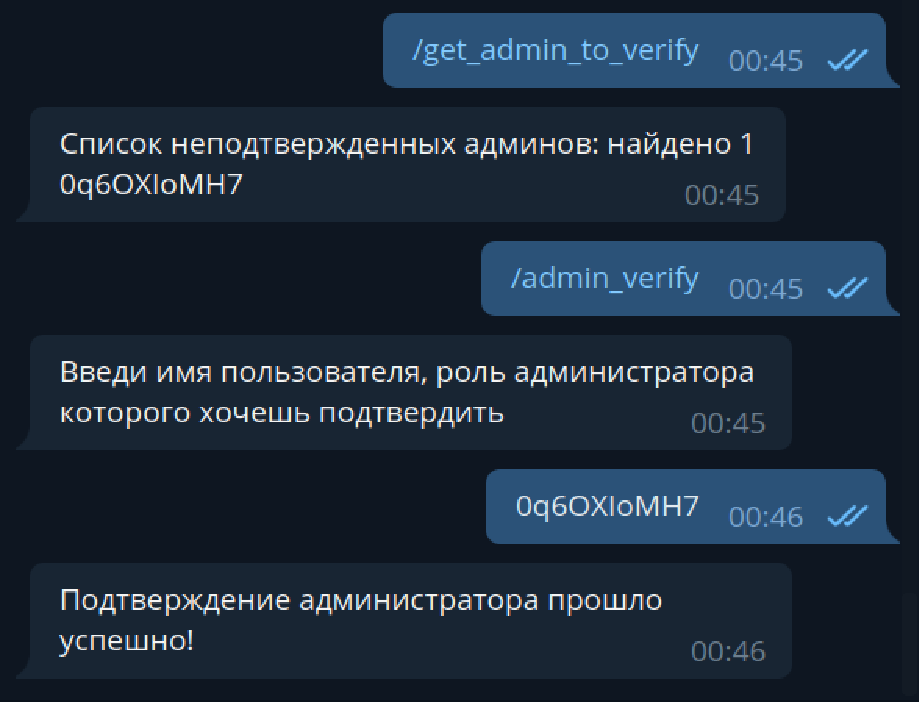
\includegraphics[page=1,scale=0.5]{assets/admin_verify.pdf}
	\end{center}
	\caption{Интерфейс подтверждения роли администратора}
	\label{admin_verify}
\end{figure}

\section{Вывод из раздела}

В данном разделе был сделан выбор СУБД и средств реализации, описано создание БД, триггера, ролей с выделением прав. Также были представлены описание генерации данных для наполнения базы и пользовательский интерфейс доступных в приложении действий.